% questions.tex —— 1986 年·全国卷·理科 · 题目内容片段（无答案）
% 由 tools/generate_projects.py 依来源总账自 1986/1986_数学真题_全国理_试题.md 生成，勿手改（改源 MD 后重跑）


\gkpart{理科数学}

\begin{gktip}
\textbf{来源说明}：本题面依据固定源 PDF《1986 年普通高等学校招生考试（全国卷）·理科数学》单页逐题转录。固定源原卷页码为 27；该 PDF 不含答案页，下列答案和解析由本库独立推导，不声称代表官方发布版本。

\textbf{图形说明}：第 8、9、17、19 题的原卷图形依据固定源图形关系重绘为 TikZ 矢量图。

\textbf{题面异文说明}：第 20 题固定源扫描字面写为“集合 $A$ 和集合 $B$ 各含有 12 个元素，$A\cup B$ 含有 4 个元素”，但两个独立公开题源/解析资料均记为 $A\cap B$ 并给出答案 $1084$。规范转录采用经交叉核定的 $A\cap B$；固定源差异及来源校验见 ISSUE-0766。
\end{gktip}

\begin{question}
\gkti{1}在下列各数中，已表示成三角形式的复数是\mbox{（　　）}

（A）$2\left(\cos\frac\pi4-i\sin\frac\pi4\right)$

（B）$2\left(\cos\frac\pi4+i\sin\frac\pi4\right)$

（C）$2\left(\sin\frac\pi4+i\cos\frac\pi4\right)$

（D）$-2\left(\sin\frac\pi4-i\cos\frac\pi4\right)$

\end{question}
\begin{question}
\gkti{2}函数

\nopagebreak[4]
\[
y=(0.2)^{-x}+1
\]

的反函数是\mbox{（　　）}

（A）$y=\log_5(x+1)$　　（B）$y=\log_x5+1$

（C）$y=\log_5(x-1)$　　（D）$y=\log_5x-1$

\end{question}
\begin{question}
\gkti{3}极坐标方程

\nopagebreak[4]
\[
\rho\cos\theta=\frac43
\]

表示\mbox{（　　）}

（A）一条平行于 $x$ 轴的直线　　（B）一条垂直于 $x$ 轴的直线

（C）一个圆　　（D）一条抛物线

\end{question}
\begin{question}
\gkti{4}函数

\nopagebreak[4]
\[
y=\sqrt2\sin2x\cos2x
\]

是\mbox{（　　）}

（A）周期为 $\dfrac\pi2$ 的奇函数　　（B）周期为 $\dfrac\pi2$ 的偶函数

（C）周期为 $\dfrac\pi4$ 的奇函数　　（D）周期为 $\dfrac\pi4$ 的偶函数

\end{question}
\begin{question}
\gkti{5}给出 20 个数：

\nopagebreak[4]
\[
87,\ 91,\ 94,\ 88,\ 93,\ 91,\ 89,\ 87,\ 92,\ 86,\ 90,\ 92,\ 88,\ 90,\ 91,
86,\ 89,\ 92,\ 95,\ 88,
\]

它们的和是\mbox{（　　）}

（A）1789　　（B）1799　　（C）1879　　（D）1899

\end{question}
\begin{question}
\gkti{6}设甲是乙的充分条件，乙是丙的充要条件，丙是丁的必要条件，那么丁是甲的\mbox{（　　）}

（A）充分条件　　（B）必要条件　　（C）充要条件　　（D）既不充分也不必要的条件

\end{question}
\begin{question}
\gkti{7}如果方程

\nopagebreak[4]
\[
x^2+y^2+Dx+Ey+F=0\ (D^2+E^2-4F>0)
\]

所表示的曲线关于直线 $y=x$ 对称，那么必有\mbox{（　　）}

（A）$D=E$　　（B）$D=F$　　（C）$E=F$　　（D）$D=E=F$

\Needspace{0.4\textheight}
\end{question}
\begin{question}
\gkti{8}在正方形 $SG_1G_2G_3$ 中，$E\text{、}F$ 分别是 $G_1G_2$ 及 $G_2G_3$ 的中点，$D$ 是 $EF$ 的中点，现在沿 $SE\text{、}SF$ 及 $EF$ 把这个正方形折成一个四面体，使 $G_1\text{、}G_2\text{、}G_3$ 三点重合，重合后的点记为 $G$，那么，在四面体 $S-EFG$ 中必有\mbox{（　　）}
\nopagebreak[4]
\begin{center}% 1986 年全国卷理科第 8 题：正方形折叠示意图
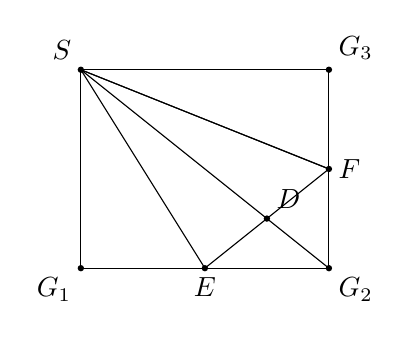
\begin{tikzpicture}[scale=1.05,>=stealth]
  \coordinate (S) at (0,2.4);
  \coordinate (G3) at (3,2.4);
  \coordinate (G2) at (3,0);
  \coordinate (G1) at (0,0);
  \coordinate (E) at (1.5,0);
  \coordinate (F) at (3,1.2);
  \coordinate (D) at (2.25,0.6);
  \draw (S)--(G3)--(G2)--(G1)--cycle;
  \draw (S)--(E)--(F)--cycle;
  \draw (S)--(F);
  \draw (S)--(G2);
  \draw (E)--(G2);
  \draw (F)--(G3);
  \fill (S) circle (1.1pt) node[above left] {$S$};
  \fill (G3) circle (1.1pt) node[above right] {$G_3$};
  \fill (G2) circle (1.1pt) node[below right] {$G_2$};
  \fill (G1) circle (1.1pt) node[below left] {$G_1$};
  \fill (E) circle (1.1pt) node[below] {$E$};
  \fill (F) circle (1.1pt) node[right] {$F$};
  \fill (D) circle (1.1pt) node[above right] {$D$};
\end{tikzpicture}
\end{center}
\nopagebreak[4]
（A）$SG\perp\triangle EFG$ 所在平面　　（B）$SD\perp\triangle EFG$ 所在平面

（C）$GF\perp\triangle SEF$ 所在平面　　（D）$GD\perp\triangle SEF$ 所在平面

\Needspace{0.4\textheight}
\end{question}
\begin{question}
\gkti{9}在下列各图中，$y=ax^2+bx$ 与 $y=ax+b$（$ab\ne0$）的图象只可能是\mbox{（　　）}
\nopagebreak[4]
\begin{center}% 1986 年全国卷理科第 9 题：四个函数图象选项
\begin{tikzpicture}[scale=0.72,>=stealth]
  \foreach \dx/\dy/\lab/\curve/\line in {
    0/2.25/{（A）}/{1.55*(\x+0.45)^2-0.55}/{0.85*\x+0.55},
    3.15/2.25/{（B）}/{1.55*\x*\x-1.55*\x}/{-0.85*\x+0.80},
    0/0/{（C）}/{-1.45*\x*\x+1.45*\x}/{-0.72*\x+0.85},
    3.15/0/{（D）}/{-1.45*\x*\x+1.45*\x}/{0.72*\x-0.55}
  } {
    \begin{scope}[shift={(\dx,\dy)}]
      \draw[->] (-1.35,0)--(1.45,0) node[right] {$x$};
      \draw[->] (0,-1.35)--(0,1.45) node[above] {$y$};
      \draw[thick,domain=-1.15:1.15,samples=80]
        plot (\x,{\curve});
      \draw[thick,domain=-1.25:1.25]
        plot (\x,{\line});
      \node[below] at (0,-1.65) {\lab};
      \node[below left] at (0,0) {$O$};
    \end{scope}
  }
\end{tikzpicture}
\end{center}
\nopagebreak[4]
\end{question}
\begin{question}
\gkti{10}当 $x\in[-1,0]$ 时，在下面关系式中正确的是\mbox{（　　）}

（A）$\pi-\arccos(-x)=\arcsin\sqrt{1-x^2}$

（B）$\pi-\arcsin(-x)=\arccos\sqrt{1-x^2}$

（C）$\pi-\arccos x=\arcsin\sqrt{1-x^2}$

（D）$\pi-\arcsin x=\arccos\sqrt{1-x^2}$

\end{question}
\begin{question}
\gkti{11}求方程

\nopagebreak[4]
\[
\sqrt{25^{(x^2+x-0.5)}}=\sqrt[4]{5}
\]

的解。

\end{question}
\begin{question}
\gkti{12}已知

\nopagebreak[4]
\[
\omega=\frac{-1-\sqrt3i}{2},
\]

求 $\omega^2+\omega+1$ 的值。

\end{question}
\begin{question}
\gkti{13}在 $xOy$ 平面上，四边形 $ABCD$ 的四个顶点坐标依次为 $(0,0)\text{、}(1,0)\text{、}(2,1)$ 及 $(0,3)$，求这个四边形绕 $x$ 轴旋转一周所得到的几何体的体积。

\end{question}
\begin{question}
\gkti{14}求

\nopagebreak[4]
\[
\lim_{n\to\infty}\frac{3^n+(-2)^n}{3^{n+1}+(-2)^{n+1}}.
\]

\end{question}
\begin{question}
\gkti{15}求

\nopagebreak[4]
\[
\left(2x^3-\frac1{x^2}\right)^5
\]

展开式中的常数项。

\end{question}
\begin{question}
\gkti{16}已知 $\sin\theta-\cos\theta=\dfrac12$，求 $\sin^3\theta-\cos^3\theta$ 的值。

\Needspace{0.4\textheight}
\end{question}
\begin{question}
\gkti{17}如图，$AB$ 是圆 $O$ 的直径，$PA$ 垂直于圆 $O$ 所在的平面，$C$ 是圆周上不同于 $A\text{、}B$ 的任一点，求证：平面 $PAC$ 垂直于平面 $PBC$。
\nopagebreak[4]
\begin{center}% 1986 年全国卷理科第 17 题：圆的直径与三棱锥示意图
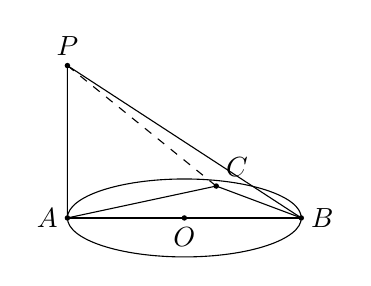
\begin{tikzpicture}[scale=0.9,>=stealth]
  \draw (0,0) ellipse (1.65 and 0.55);
  \draw[dashed] (-1.65,0)--(1.65,0);
  \draw (-1.65,0)--(1.65,0);
  \fill (0,0) circle (1.1pt) node[below] {$O$};
  \fill (-1.65,0) circle (1.1pt) node[left] {$A$};
  \fill (1.65,0) circle (1.1pt) node[right] {$B$};
  \coordinate (C) at (0.45,0.45);
  \fill (C) circle (1.1pt) node[above right] {$C$};
  \coordinate (P) at (-1.65,2.15);
  \fill (P) circle (1.1pt) node[above] {$P$};
  \draw (P)--(-1.65,0);
  \draw (P)--(1.65,0);
  \draw[dashed] (P)--(C);
  \draw (C)--(-1.65,0);
  \draw (C)--(1.65,0);
\end{tikzpicture}
\end{center}
\nopagebreak[4]
\end{question}
\begin{question}
\gkti{18}当 $\sin2x>0$，求不等式

\nopagebreak[4]
\[
\log_{0.5}(x^2-2x-15)>\log_{0.5}(x+13)
\]

的解集。

\Needspace{0.4\textheight}
\end{question}
\begin{question}
\gkti{19}如图，在平面直角坐标系中，在 $y$ 轴的正半轴（坐标原点除外）上给定两点 $A\text{、}B$ 试在 $x$ 轴的正半轴（坐标原点除外）上求点 $C$，使 $\angle ACB$ 取得最大值。
\nopagebreak[4]
\begin{center}% 1986 年全国卷理科第 19 题：最大角示意图
\begin{tikzpicture}[scale=0.95,>=stealth]
  \draw[->] (-0.2,0)--(4.0,0) node[right] {$x$};
  \draw[->] (0,-0.2)--(0,3.5) node[above] {$y$};
  \coordinate (A) at (0,3.0);
  \coordinate (B) at (0,1.45);
  \coordinate (C) at (2.1,0);
  \fill (A) circle (1.1pt) node[left] {$A$};
  \fill (B) circle (1.1pt) node[left] {$B$};
  \fill (C) circle (1.1pt) node[below] {$C$};
  \fill (0,0) circle (1.1pt) node[below left] {$O$};
  \draw (A)--(C)--(B);
\end{tikzpicture}
\end{center}
\nopagebreak[4]
\end{question}
\begin{question}
\gkti{20}已知集合 $A$ 和集合 $B$ 各含有 12 个元素，$A\cap B$ 含有 4 个元素，试求同时满足下面两个条件的集合 $C$ 的个数：

（1）$C\subseteq A\cup B$ 且 $C$ 中含有 3 个元素；

（2）$C\cap A\ne\varnothing$（$\varnothing$ 表示空集）。

\end{question}
\begin{question}
\gkti{21}过点 $M(-1,0)$ 的直线 $L_1$ 与抛物线

\nopagebreak[4]
\[
y^2=4x
\]

交于 $P_1\text{、}P_2$ 两点。记：线段 $P_1P_2$ 的中点为 $P$；过点 $P$ 和这个抛物线的焦点 $F$ 的直线为 $L_2$；$L_1$ 的斜率为 $k$。试把直线 $L_2$ 的斜率与直线 $L_1$ 的斜率之比表示为 $k$ 的函数，并指出这个函数的定义域、单调区间，同时说明在每一单调区间上它是增函数还是减函数。

\end{question}
\begin{question}
\gkti{22}已知 $x_1>0$，$x_1\ne1$，且

\nopagebreak[4]
\[
x_{n+1}=\frac{x_n(x_n^2+3)}{3x_n^2+1},\ (n=1,2,\cdots).
\]

试证：数列 $\{x_n\}$ 或者对任意自然数 $n$ 都满足 $x_n<x_{n+1}$，或者对任意自然数 $n$ 都满足 $x_n>x_{n+1}$。

\Needspace{0.25\textheight}
\textbf{附加题}

\end{question}
\begin{question}
\gkti{23}求

\nopagebreak[4]
\[
y=x\arctan x^2
\]

的导数。

\end{question}
\begin{question}
\gkti{24}求过点 $(-1,0)$ 并与曲线

\nopagebreak[4]
\[
y=\frac{x+1}{x+2}
\]

相切的直线方程。

\end{question}